\documentclass[a4paper,12pt]{article}
\usepackage[top = 2.5cm, bottom = 2.5cm, left = 2.5cm, right = 2.5cm]{geometry}
\usepackage[T1]{fontenc}
\usepackage[utf8]{inputenc}
\usepackage{multirow} 
\usepackage{booktabs} 
\usepackage{graphicx}
\usepackage[spanish]{babel}
\usepackage{setspace}
\setlength{\parindent}{0in}
\usepackage{float}
\usepackage{fancyhdr}
\usepackage{amsmath}
\usepackage{amssymb}
\usepackage{amsthm}
\usepackage[numbers]{natbib}
\newcommand\Mycite[1]{%
	\citeauthor{#1}~[\citeyear{#1}]}
\usepackage{graphicx}
\usepackage{subcaption}
\usepackage{booktabs}
\usepackage{etoolbox}
\usepackage{minibox}
\usepackage{hyperref}
\usepackage{xcolor}
\usepackage[skins]{tcolorbox}
%---------------------------

\newtcolorbox{cajita}[1][]{
	 #1
}

\newenvironment{sol}
{\renewcommand\qedsymbol{$\square$}\begin{proof}[\textbf{Solución.}]}
	{\end{proof}}

\newenvironment{dem}
{\renewcommand\qedsymbol{$\blacksquare$}\begin{proof}[\textbf{Demostración.}]}
	{\end{proof}}

\newtheorem{problema}{Problema}
\newtheorem{definicion}{Definición}
\newtheorem{ejemplo}{Ejemplo}
\newtheorem{teorema}{Teorema}
\newtheorem{corolario}{Corolario}[teorema]
\newtheorem{lema}[teorema]{Lema}
\newtheorem{prop}{Proposición}
\newtheorem*{nota}{\textbf{NOTA}}
\renewcommand\qedsymbol{$\blacksquare$}
\usepackage{svg}
\usepackage{pgfplots}
\pgfplotsset{compat=1.11}

\usepackage{tikz}
\usetikzlibrary{calc}

\usetikzlibrary{patterns}
\usepackage[framemethod=default]{mdframed}
\global\mdfdefinestyle{exampledefault}{%
linecolor=lightgray,linewidth=1pt,%
leftmargin=1cm,rightmargin=1cm,
}




\newenvironment{noter}[1]{%
\mdfsetup{%
frametitle={\tikz\node[fill=white,rectangle,inner sep=0pt,outer sep=0pt]{#1};},
frametitleaboveskip=-0.5\ht\strutbox,
frametitlealignment=\raggedright
}%
\begin{mdframed}[style=exampledefault]
}{\end{mdframed}}
\newcommand{\linea}{\noindent\rule{\textwidth}{3pt}}
\newcommand{\linita}{\noindent\rule{\textwidth}{1pt}}

\AtBeginEnvironment{align}{\setcounter{equation}{0}}
\pagestyle{fancy}

\fancyhf{}









%----------------------------------------------------------
\lhead{\footnotesize Geometría diferencial}
\rhead{\footnotesize  Rudik Roberto Rompich}
\cfoot{\footnotesize \thepage}


%--------------------------

\begin{document}
 \thispagestyle{empty} 
    \begin{tabular}{p{15.5cm}}
    \begin{tabbing}
    \textbf{Universidad del Valle de Guatemala} \\
    Departamento de Matemática\\
    Licenciatura en Matemática Aplicada\\\\
   \textbf{Estudiante:} Rudik Roberto Rompich\\
   \textbf{Correo:}  \href{mailto:rom19857@uvg.edu.gt}{rom19857@uvg.edu.gt}\\
   \textbf{Carné:} 19857
    \end{tabbing}
    \begin{center}
        Geometría diferencial - Catedrático: Alan Reyes\\
        \today
    \end{center}\\
    \hline
    \\
    \end{tabular} 
    \vspace*{0.3cm} 
    \begin{center} 
    {\Large \bf  Tarea
} 
        \vspace{2mm}
    \end{center}
    \vspace{0.4cm}
%--------------------------
\section{Introducción}
En este informe presentamos y discutimos los resultados de nuestro script en Python que calcula y grafica la ecuación:

\begin{equation}
V(x, y) = \frac{4V_0}{\pi}\sum_{n=1,3,5,7,9}\frac{ \sin \left(\frac{n \pi x}{b}\right) \sinh \left(\frac{n \pi y}{b}\right)}{n \sinh \left(\frac{n \pi a}{b}\right)}
\end{equation}
El objetivo es:
\begin{itemize}
    \item Calcular los valores de V(x,y) utilizando la ecuación anterior al utilizar los primeros 5 términos de la sumatoria.
    \item Graficar los valores V(x,y) para 5 escenarios.
\end{itemize}

\section{Desarrollo del programa}

Usamos Python para realizar la simulación, para esto hicimos uso de los siguientes paquetes: 
\begin{verbatim}
    import numpy as np
    import pandas as pd
    import matplotlib.pyplot as plt
    from mpl_toolkits.mplot3d import Axes3D
\end{verbatim}
Posteriormente a esto, modelamos la ecuación (1) para generar los valores de $V$ datos dos valores iniciales $(x,y)$, dados unos $a,b,V_0$ iniciales con la siguiente función: 
\begin{verbatim}
def v(x,y,a,b,v_0):
    suma = 0
    for n in range(1,10,2):
        suma= suma+ np.sin((n*np.pi*x)/b)*np.sinh((n*np.pi*y)/b)/
              (n*np.sinh((n*np.pi*a)/b))
    return ((4*v_0)/np.pi)*suma
\end{verbatim} 
Por otra parte, creamos una función para generar las tablas con los nuevos valores de $V(x,y)$,
\begin{verbatim}
def generador_dataframe(data):
    df = pd.DataFrame(data)
    df['v(x,y)'] = v(df['X'], df['y'], df['a'], df['B'], df['Vo'])
    return df
\end{verbatim}
Por último, procedimos a crear una función para graficar los resultados, 
\begin{verbatim}
def create_plot(df):
    fig = plt.figure(figsize=(10, 7))
    ax = fig.add_subplot(111, projection='3d')

    ax.scatter(df['X'], df['y'], df['v(x,y)'])

    ax.set_xlabel('X')
    ax.set_ylabel('Y')
    ax.set_zlabel('v(x,y)')

    plt.show()
\end{verbatim}

Con esto, transformamos los datos originales al formato correcto y usamos las funciones, de esto obtuvimos los siguientes datos, con sus respectivas gráficas: 

\begin{itemize}
    \item Datos 1
    \begin{center}
        \begin{tabular}{lcccccc}
            & X & y & a & B & Vo & v(x,y) \\
           0 & 0.250000 & 0.250000 & 1 & 1 & 100 & 6.797167 \\
           1 & 0.250000 & 0.500000 & 1 & 1 & 100 & 18.202833 \\
           2 & 0.250000 & 0.750000 & 1 & 1 & 100 & 43.201676 \\
           3 & 0.500000 & 0.250000 & 1 & 1 & 100 & 9.541412 \\
           4 & 0.500000 & 0.500000 & 1 & 1 & 100 & 25.000000 \\
           5 & 0.500000 & 0.750000 & 1 & 1 & 100 & 54.054665 \\
           6 & 0.750000 & 0.250000 & 1 & 1 & 100 & 6.797167 \\
           7 & 0.750000 & 0.500000 & 1 & 1 & 100 & 18.202833 \\
           8 & 0.750000 & 0.750000 & 1 & 1 & 100 & 43.201676 \\
           \end{tabular}
           
    \end{center}
    \begin{figure}[H]
        \centering
        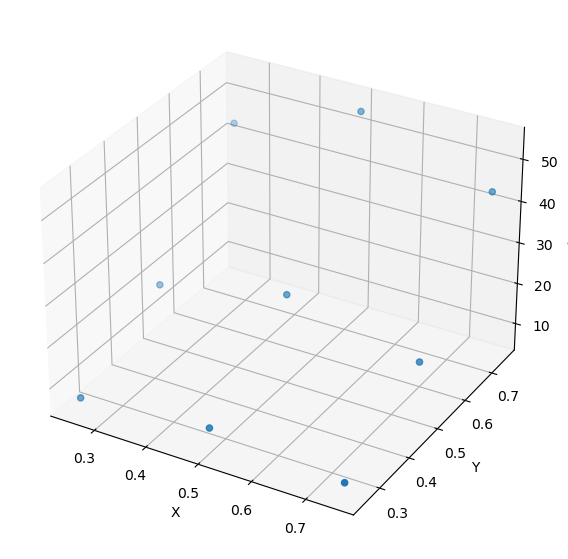
\includegraphics[scale=0.5]{Problemas/1.png}
    \end{figure}
    \item Datos 2 
    \begin{center}
        \begin{tabular}{lcccccc}
            & X & y & a & B & Vo & v(x,y) \\
           0 & 0.250000 & 0.250000 & 1 & 2 & 100 & 9.631115 \\
           1 & 0.250000 & 0.500000 & 1 & 2 & 100 & 22.562696 \\
           2 & 0.250000 & 0.750000 & 1 & 2 & 100 & 46.779384 \\
           3 & 0.500000 & 0.250000 & 1 & 2 & 100 & 16.501962 \\
           4 & 0.500000 & 0.500000 & 1 & 2 & 100 & 36.404509 \\
           5 & 0.500000 & 0.750000 & 1 & 2 & 100 & 63.689151 \\
           6 & 0.750000 & 0.250000 & 1 & 2 & 100 & 20.141519 \\
           7 & 0.750000 & 0.500000 & 1 & 2 & 100 & 42.742626 \\
           8 & 0.750000 & 0.750000 & 1 & 2 & 100 & 69.477914 \\
           \end{tabular}
    \end{center}
    \begin{figure}[H]
        \centering
        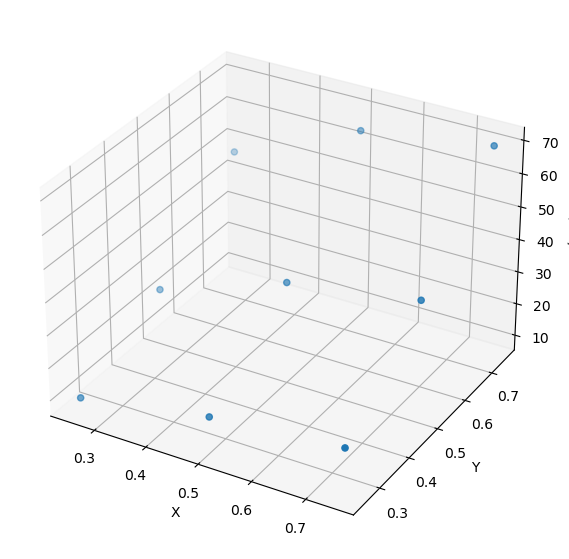
\includegraphics[scale=0.5]{Problemas/2.png}
    \end{figure}
    \item Datos 3 
    \begin{center}
        \begin{tabular}{lcccccc}
            & X & y & a & B & Vo & v(x,y) \\
           0 & 0.250000 & 0.250000 & 1 & 3 & 100 & 9.769669 \\
           1 & 0.250000 & 0.500000 & 1 & 3 & 100 & 22.754744 \\
           2 & 0.250000 & 0.750000 & 1 & 3 & 100 & 46.898063 \\
           3 & 0.500000 & 0.250000 & 1 & 3 & 100 & 16.869678 \\
           4 & 0.500000 & 0.500000 & 1 & 3 & 100 & 36.937458 \\
           5 & 0.500000 & 0.750000 & 1 & 3 & 100 & 64.117838 \\
           6 & 0.750000 & 0.250000 & 1 & 3 & 100 & 20.967512 \\
           7 & 0.750000 & 0.500000 & 1 & 3 & 100 & 43.913690 \\
           8 & 0.750000 & 0.750000 & 1 & 3 & 100 & 70.212130 \\
           \end{tabular}
    \end{center}
    \begin{figure}[H]
        \centering
        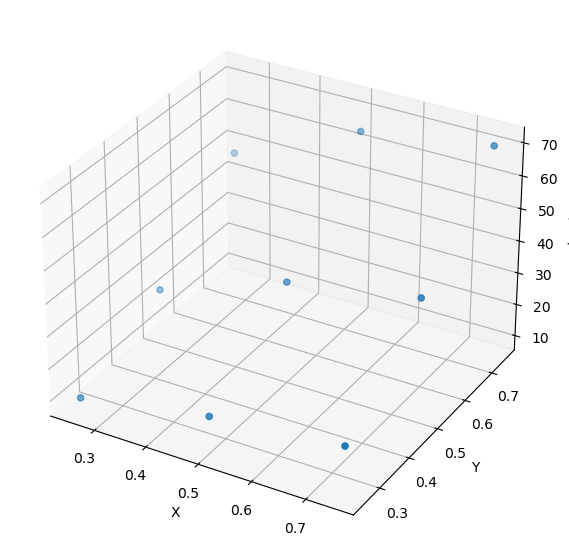
\includegraphics[scale=0.5]{Problemas/3.png}
    \end{figure}
    \item Datos 4 
    \begin{center}
        \begin{tabular}{lcccccc}
            & X & y & a & B & Vo & v(x,y) \\
           0 & 0.250000 & 0.250000 & 1 & 4 & 100 & 9.758862 \\
           1 & 0.250000 & 0.500000 & 1 & 4 & 100 & 22.606970 \\
           2 & 0.250000 & 0.750000 & 1 & 4 & 100 & 45.447219 \\
           3 & 0.500000 & 0.250000 & 1 & 4 & 100 & 16.905571 \\
           4 & 0.500000 & 0.500000 & 1 & 4 & 100 & 37.148269 \\
           5 & 0.500000 & 0.750000 & 1 & 4 & 100 & 65.926464 \\
           6 & 0.750000 & 0.250000 & 1 & 4 & 100 & 20.996643 \\
           7 & 0.750000 & 0.500000 & 1 & 4 & 100 & 43.889038 \\
           8 & 0.750000 & 0.750000 & 1 & 4 & 100 & 69.437827 \\
           \end{tabular}
    \end{center}
    \begin{figure}[H]
        \centering
        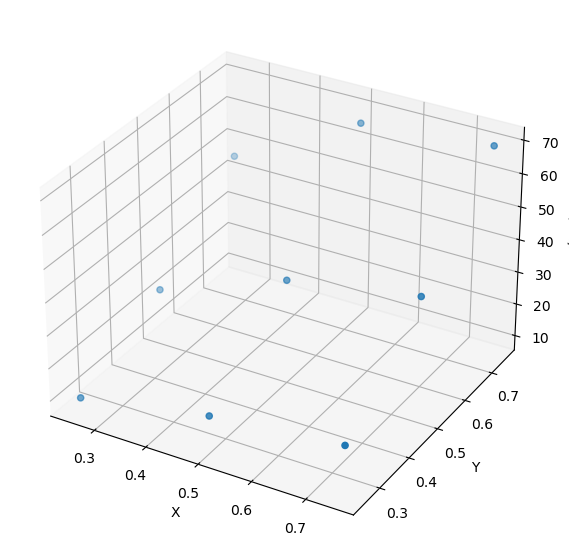
\includegraphics[scale=0.5]{Problemas/4.png}
    \end{figure}
    \item Datos 5
    \begin{center}
        \begin{tabular}{lcccccc}
            & X & y & a & B & Vo & v(x,y) \\
           0 & 0.250000 & 0.250000 & 1 & 5 & 100 & 9.689333 \\
           1 & 0.250000 & 0.500000 & 1 & 5 & 100 & 22.192581 \\
           2 & 0.250000 & 0.750000 & 1 & 5 & 100 & 43.045762 \\
           3 & 0.500000 & 0.250000 & 1 & 5 & 100 & 16.931233 \\
           4 & 0.500000 & 0.500000 & 1 & 5 & 100 & 37.300042 \\
           5 & 0.500000 & 0.750000 & 1 & 5 & 100 & 66.814483 \\
           6 & 0.750000 & 0.250000 & 1 & 5 & 100 & 21.058218 \\
           7 & 0.750000 & 0.500000 & 1 & 5 & 100 & 44.246208 \\
           8 & 0.750000 & 0.750000 & 1 & 5 & 100 & 71.486005 \\
           \end{tabular}
    \end{center}
    \begin{figure}[H]
        \centering
        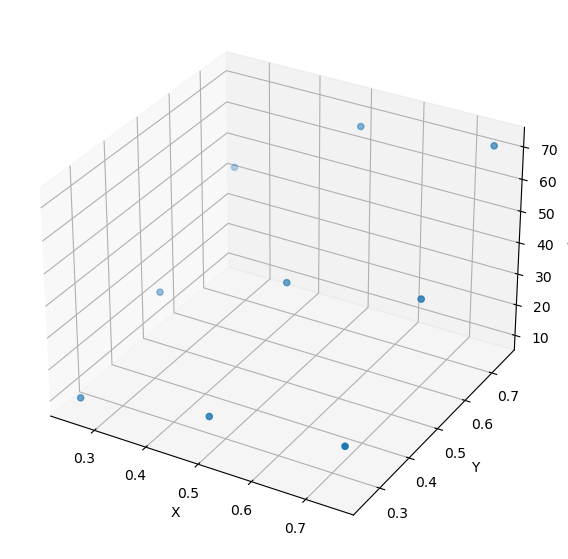
\includegraphics[scale=0.5]{Problemas/5.png}
    \end{figure}
\end{itemize}

\section{Discusión}

En base a los resultados obtenidos a partir de las cinco simulaciones, es posible notar que existen variaciones en los valores de $V(x,y)$ en función de las diferentes combinaciones de parámetros. Los cambios son perceptibles tanto en los valores de la tabla como en las gráficas.\bigbreak

De las tablas, podemos observar que el valor de $V(x, y)$ tiende a incrementar conforme aumenta el valor de $y$, para un $x$ fijo. De igual manera, $V(x, y)$ aumenta cuando $x$ crece, para un $y$ fijo. Sin embargo, este incremento no es lineal debido a las funciones trigonométricas y de hiperboloide presentes en la ecuación.\bigbreak

En cuanto a las gráficas, notamos que la representación de la ecuación en un espacio tridimensional permite visualizar de manera más clara el comportamiento de la función. Al observar las gráficas, se puede notar que el aumento de $V(x, y)$ se asemeja a una superficie curvada en tres dimensiones, evidenciando la no linealidad de la función.\bigbreak

Una observación adicional es que los valores de $V(x, y)$ aumentan conforme $B$ se incrementa. Esto se puede deber a que $B$ afecta directamente a los valores dentro de las funciones trigonométricas y de hiperboloide, amplificando o reduciendo la influencia de estos términos en el resultado final.

\section{Conclusiones}

A partir de las simulaciones realizadas y de la discusión de los resultados, es posible concluir que el comportamiento de $V(x, y)$ es altamente dependiente de las combinaciones de parámetros de entrada.\bigbreak

Además, el uso de un script en Python para realizar estas simulaciones resultó ser una herramienta eficaz para el análisis de esta ecuación. La posibilidad de cambiar los parámetros de entrada con facilidad y obtener tanto los valores tabulares como las representaciones gráficas de los resultados, permitieron un mejor entendimiento del comportamiento de la función.\bigbreak

El estudio de esta ecuación con múltiples sets de parámetros provee información valiosa para entender cómo las variables de entrada afectan el resultado final de $V(x,y)$. Adicionalmente, la visualización tridimensional de los datos ofrece una perspectiva más intuitiva sobre la no linealidad de la función y cómo ésta se ve afectada por los diferentes parámetros.\bigbreak

Finalmente, es importante mencionar que este estudio es útil para proporcionar una base sólida para futuras investigaciones o aplicaciones que hagan uso de esta ecuación o similares, ya que brinda un entendimiento más profundo sobre su comportamiento y sobre las implicancias de las variaciones en sus parámetros.

\section{Programa}

\begin{verbatim}
import numpy as np
import pandas as pd
import matplotlib.pyplot as plt
from mpl_toolkits.mplot3d import Axes3D

def v(x,y,a,b,v_0):
    suma = 0
    for n in range(1,10,2):
        suma= suma+ np.sin((n*np.pi*x)/b)*np.sinh((n*np.pi*y)/b)/
              (n*np.sinh((n*np.pi*a)/b))
    return ((4*v_0)/np.pi)*suma


data_1 = {
    "X": [0.25, 0.25, 0.25, 0.50, 0.50, 0.50, 0.75, 0.75, 0.75],
    "y": [0.25, 0.50, 0.75, 0.25, 0.50, 0.75, 0.25, 0.50, 0.75],
    "a": [1, 1, 1, 1, 1, 1, 1, 1, 1],
    "B": [1, 1, 1, 1, 1, 1, 1, 1, 1],
    "Vo": [100, 100, 100, 100, 100, 100, 100, 100, 100]
}

data_2 = {
    "X": [0.25, 0.25, 0.25, 0.50, 0.50, 0.50, 0.75, 0.75, 0.75],
    "y": [0.25, 0.50, 0.75, 0.25, 0.50, 0.75, 0.25, 0.50, 0.75],
    "a": [1, 1, 1, 1, 1, 1, 1, 1, 1],
    "B": [2, 2, 2, 2, 2, 2, 2, 2, 2],
    "Vo": [100, 100, 100, 100, 100, 100, 100, 100, 100]
}

data_3 = {
    "X": [0.25, 0.25, 0.25, 0.50, 0.50, 0.50, 0.75, 0.75, 0.75],
    "y": [0.25, 0.50, 0.75, 0.25, 0.50, 0.75, 0.25, 0.50, 0.75],
    "a": [1, 1, 1, 1, 1, 1, 1, 1, 1],
    "B": [3, 3, 3, 3, 3, 3, 3, 3, 3],
    "Vo": [100, 100, 100, 100, 100, 100, 100, 100, 100]
}


data_4 = {
    "X": [0.25, 0.25, 0.25, 0.50, 0.50, 0.50, 0.75, 0.75, 0.75],
    "y": [0.25, 0.50, 0.75, 0.25, 0.50, 0.75, 0.25, 0.50, 0.75],
    "a": [1, 1, 1, 1, 1, 1, 1, 1, 1],
    "B": [4, 4, 4, 4, 4, 4, 4, 4, 4],
    "Vo": [100, 100, 100, 100, 100, 100, 100, 100, 100]
}

data_5 = {
    "X": [0.25, 0.25, 0.25, 0.50, 0.50, 0.50, 0.75, 0.75, 0.75],
    "y": [0.25, 0.50, 0.75, 0.25, 0.50, 0.75, 0.25, 0.50, 0.75],
    "a": [1, 1, 1, 1, 1, 1, 1, 1, 1],
    "B": [5, 5, 5, 5, 5, 5, 5, 5, 5],
    "Vo": [100, 100, 100, 100, 100, 100, 100, 100, 100]
}


def create_plot(df):
    fig = plt.figure(figsize=(10, 7))
    ax = fig.add_subplot(111, projection='3d')

    ax.scatter(df['X'], df['y'], df['v(x,y)'])

    ax.set_xlabel('X')
    ax.set_ylabel('Y')
    ax.set_zlabel('v(x,y)')

    plt.show()
    
    
def generador_dataframe(data):
    df = pd.DataFrame(data)
    df['v(x,y)'] = v(df['X'], df['y'], df['a'], df['B'], df['Vo'])
    return df



# Generador data, unicamente se edita el input de generador_dataframe()
data_final = generador_dataframe(data_5)
print(data_final.style.to_latex(column_format='lcccccc'))
create_plot(data_final)

\end{verbatim}
%---------------------------
%\bibliographystyle{apa}
%\bibliography{referencias.bib}

\end{document}